\documentclass[10pt]{article}
\usepackage[a3paper,landscape,margin=1.0cm]{geometry}
\usepackage{tikz}
\usetikzlibrary{arrows.meta,positioning,shadows}
\usepackage[T1]{fontenc}
\usepackage{helvet}
\renewcommand{\familydefault}{\sfdefault}
\usepackage{xcolor}
\usepackage{graphicx}
\pagestyle{empty}

\definecolor{ink}{HTML}{24292F}
\definecolor{muted}{HTML}{57606A}
\definecolor{ok}{HTML}{1A7F37}
\definecolor{bad}{HTML}{C93C37}
\definecolor{rca}{HTML}{7A4CB8}
\definecolor{paper}{HTML}{FBFBF9}
\definecolor{lane}{HTML}{E8EAED}
\definecolor{band}{HTML}{FFF8C5}

\begin{document}
\pagecolor{paper}
\begin{center}

{\LARGE\bfseries The Timestamp Path}\\[2pt]
{\large\color{muted} How time crosses hardware, kernel, and userspace --- and how one missed egress timestamp takes a cell off the air}\\[2pt]
{\small\color{muted} Standards: ITU-T G.8275.1 (full on-path support)  $\cdot$  IEEE 1588  $\cdot$  O-RAN S-plane  $\cdot$  3GPP TS 28.532 / TS 38.104}

\vspace{4mm}

\resizebox{!}{185mm}{%
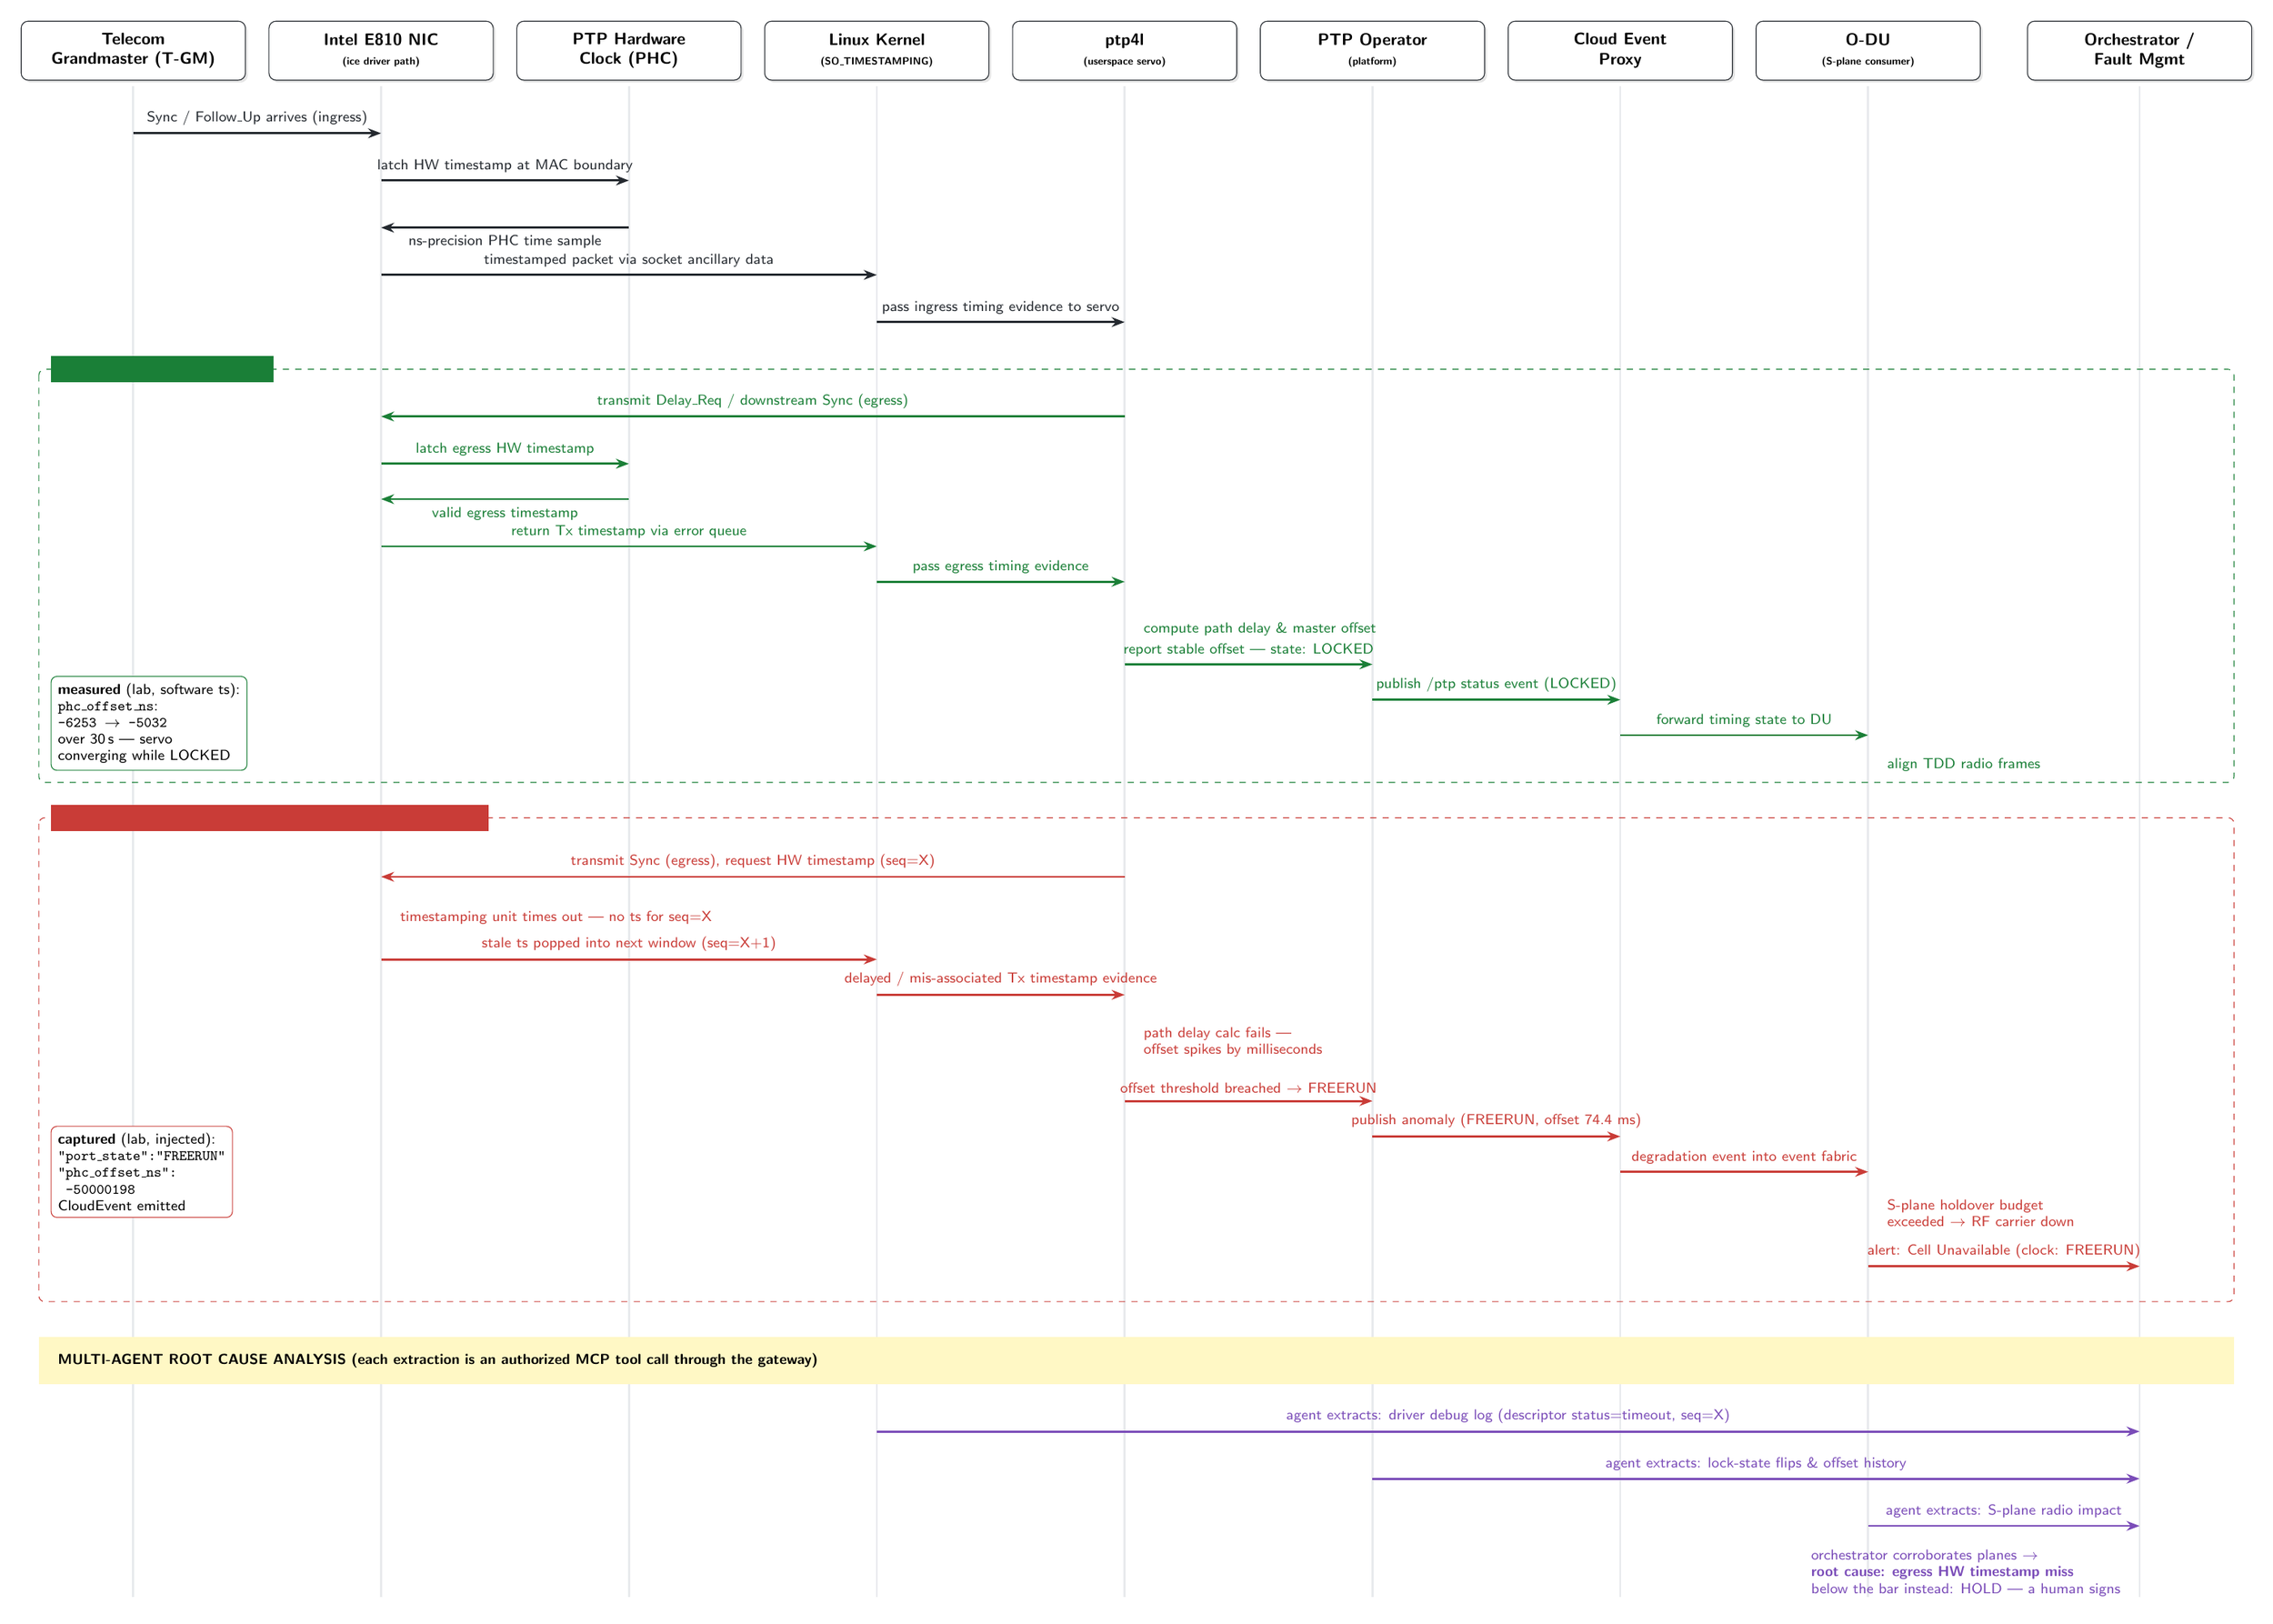
\begin{tikzpicture}[
  x=1mm, y=1mm,
  actor/.style={draw=ink, fill=white, rounded corners=1.2mm, minimum width=38mm,
                minimum height=10mm, align=center, font=\bfseries\footnotesize,
                drop shadow={shadow xshift=0.4mm, shadow yshift=-0.4mm, opacity=0.2}},
  lifeline/.style={draw=lane, line width=1.0pt},
  msg/.style={-{Stealth[length=2.2mm]}, line width=1.0pt, color=ink},
  okmsg/.style={msg, color=ok},
  badmsg/.style={msg, color=bad},
  rcamsg/.style={msg, color=rca},
  note/.style={font=\scriptsize, align=center},
  lnote/.style={font=\scriptsize, align=left},
  frame/.style={draw=muted, dashed, rounded corners=1mm},
  framelabel/.style={font=\scriptsize\bfseries, fill=white, inner sep=1mm}
]

% lifeline x positions (9 lanes)
\def\xA{0}    % T-GM
\def\xB{42}   % Intel E810 NIC
\def\xC{84}   % PHC
\def\xD{126}  % Linux kernel
\def\xE{168}  % ptp4l servo
\def\xF{210}  % PTP Operator
\def\xG{252}  % Cloud Event Proxy
\def\xH{294}  % O-DU (S-plane consumer)
\def\xI{340}  % Orchestrator / fault mgmt

\node[actor] (A) at (\xA,0)  {Telecom\\Grandmaster (T-GM)};
\node[actor] (B) at (\xB,0)  {Intel E810 NIC\\{\tiny (ice driver path)}};
\node[actor] (C) at (\xC,0)  {PTP Hardware\\Clock (PHC)};
\node[actor] (D) at (\xD,0)  {Linux Kernel\\{\tiny (SO\_TIMESTAMPING)}};
\node[actor] (E) at (\xE,0)  {ptp4l\\{\tiny (userspace servo)}};
\node[actor] (F) at (\xF,0)  {PTP Operator\\{\tiny (platform)}};
\node[actor] (G) at (\xG,0)  {Cloud Event\\Proxy};
\node[actor] (H) at (\xH,0)  {O-DU\\{\tiny (S-plane consumer)}};
\node[actor] (I) at (\xI,0)  {Orchestrator /\\Fault Mgmt};

\foreach \x in {\xA,\xB,\xC,\xD,\xE,\xF,\xG,\xH,\xI}{ \draw[lifeline] (\x,-6) -- (\x,-262); }

% ---------------- ingress (common) ----------------
\draw[msg] (\xA,-14) -- (\xB,-14) node[midway, above, note]{Sync / Follow\_Up arrives (ingress)};
\draw[msg] (\xB,-22) -- (\xC,-22) node[midway, above, note]{latch HW timestamp at MAC boundary};
\draw[msg] (\xC,-30) -- (\xB,-30) node[midway, below, note]{ns-precision PHC time sample};
\draw[msg] (\xB,-38) -- (\xD,-38) node[midway, above, note]{timestamped packet via socket ancillary data};
\draw[msg] (\xD,-46) -- (\xE,-46) node[midway, above, note]{pass ingress timing evidence to servo};

% ---------------- alt frame 1: steady state ----------------
\draw[frame, color=ok] (-16,-54) rectangle (356,-124);
\node[framelabel, color=ok, anchor=west] at (-14,-54) {NORMAL PATH (steady state)};

\draw[okmsg] (\xE,-62) -- (\xB,-62) node[midway, above, note, color=ok]{transmit Delay\_Req / downstream Sync (egress)};
\draw[okmsg] (\xB,-70) -- (\xC,-70) node[midway, above, note, color=ok]{latch egress HW timestamp};
\draw[okmsg] (\xC,-76) -- (\xB,-76) node[midway, below, note, color=ok]{valid egress timestamp};
\draw[okmsg] (\xB,-84) -- (\xD,-84) node[midway, above, note, color=ok]{return Tx timestamp via error queue};
\draw[okmsg] (\xD,-90) -- (\xE,-90) node[midway, above, note, color=ok]{pass egress timing evidence};
\node[lnote, color=ok, anchor=west] at (\xE+2,-98) {compute path delay \& master offset};
\draw[okmsg] (\xE,-104) -- (\xF,-104) node[midway, above, note, color=ok]{report stable offset --- state: LOCKED};
\draw[okmsg] (\xF,-110) -- (\xG,-110) node[midway, above, note, color=ok]{publish /ptp status event (LOCKED)};
\draw[okmsg] (\xG,-116) -- (\xH,-116) node[midway, above, note, color=ok]{forward timing state to DU};
\node[lnote, color=ok, anchor=west] at (\xH+2,-121) {align TDD radio frames};

% measured data callout
\node[lnote, draw=ok, rounded corners=1mm, fill=white, anchor=west] at (-14,-114)
  {\textbf{measured} (lab, software ts):\\ \texttt{phc\_offset\_ns}:\\ \texttt{-6253 $\to$ -5032}\\ over 30\,s --- servo\\ converging while LOCKED};

% ---------------- alt frame 2: incident ----------------
\draw[frame, color=bad] (-16,-130) rectangle (356,-212);
\node[framelabel, color=bad, anchor=west] at (-14,-130) {INCIDENT: egress HW timestamp miss (\texttt{tx\_hwtstamp\_timeout})};

\draw[badmsg] (\xE,-140) -- (\xB,-140) node[midway, above, note, color=bad]{transmit Sync (egress), request HW timestamp (seq=X)};
\node[lnote, color=bad, anchor=west] at (\xB+2,-147) {timestamping unit times out --- no ts for seq=X};
\draw[badmsg] (\xB,-154) -- (\xD,-154) node[midway, above, note, color=bad]{stale ts popped into next window (seq=X+1)};
\draw[badmsg] (\xD,-160) -- (\xE,-160) node[midway, above, note, color=bad]{delayed / mis-associated Tx timestamp evidence};
\node[lnote, color=bad, anchor=west] at (\xE+2,-168) {path delay calc fails ---\\ offset spikes by milliseconds};
\draw[badmsg] (\xE,-178) -- (\xF,-178) node[midway, above, note, color=bad]{offset threshold breached $\to$ FREERUN};
\draw[badmsg] (\xF,-184) -- (\xG,-184) node[midway, above, note, color=bad]{publish anomaly (FREERUN, offset 74.4 ms)};
\draw[badmsg] (\xG,-190) -- (\xH,-190) node[midway, above, note, color=bad]{degradation event into event fabric};
\node[lnote, color=bad, anchor=west] at (\xH+2,-197) {S-plane holdover budget\\ exceeded $\to$ RF carrier down};
\draw[badmsg] (\xH,-206) -- (\xI,-206) node[midway, above, note, color=bad]{alert: Cell Unavailable (clock: FREERUN)};

% captured data callout
\node[lnote, draw=bad, rounded corners=1mm, fill=white, anchor=west] at (-14,-190)
  {\textbf{captured} (lab, injected):\\ \texttt{"port\_state":"FREERUN"}\\ \texttt{"phc\_offset\_ns":}\\ \texttt{\ -50000198}\\ CloudEvent emitted};

% ---------------- RCA band ----------------
\fill[band] (-16,-218) rectangle (356,-226);
\node[font=\scriptsize\bfseries, anchor=west] at (-14,-222) {MULTI-AGENT ROOT CAUSE ANALYSIS (each extraction is an authorized MCP tool call through the gateway)};

\draw[rcamsg] (\xD,-234) -- (\xI,-234) node[midway, above, note, color=rca]{agent extracts: driver debug log (descriptor status=timeout, seq=X)};
\draw[rcamsg] (\xF,-242) -- (\xI,-242) node[midway, above, note, color=rca]{agent extracts: lock-state flips \& offset history};
\draw[rcamsg] (\xH,-250) -- (\xI,-250) node[midway, above, note, color=rca]{agent extracts: S-plane radio impact};
\node[lnote, color=rca, anchor=east] at (\xI-2,-258) {orchestrator corroborates planes $\to$\\ \textbf{root cause: egress HW timestamp miss}\\ below the bar instead: HOLD --- a human signs};

\end{tikzpicture}}

\vspace{3mm}

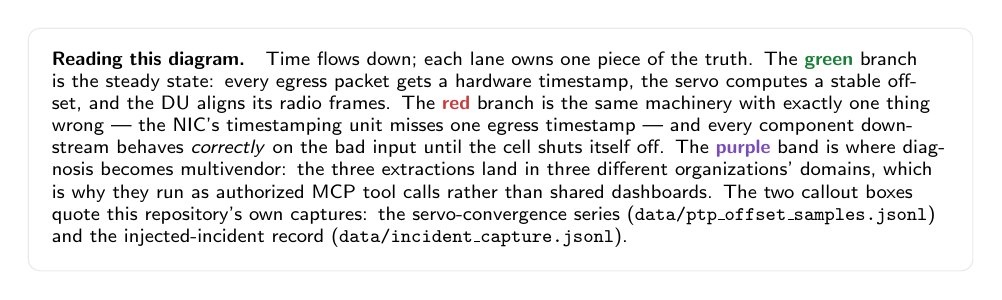
\begin{tikzpicture}[x=1mm,y=1mm]
\node[draw=lane, rounded corners=1.5mm, fill=white, inner sep=3mm, align=left, font=\scriptsize, text width=0.94\textwidth] at (0,0) {
  \textbf{Reading this diagram.}\quad Time flows down; each lane owns one piece of the truth. The
  \textcolor{ok}{\textbf{green}} branch is the steady state: every egress packet gets a hardware timestamp, the servo computes a stable offset, and the DU aligns its radio frames.
  The \textcolor{bad}{\textbf{red}} branch is the same machinery with exactly one thing wrong --- the NIC's timestamping unit misses one egress timestamp --- and every component downstream
  behaves \emph{correctly} on the bad input until the cell shuts itself off. The \textcolor{rca}{\textbf{purple}} band is where diagnosis becomes multivendor: the three extractions
  land in three different organizations' domains, which is why they run as authorized MCP tool calls rather than shared dashboards. The two callout boxes quote this repository's
  own captures: the servo-convergence series (\texttt{data/ptp\_offset\_samples.jsonl}) and the injected-incident record (\texttt{data/incident\_capture.jsonl}).
};
\end{tikzpicture}

\end{center}
\end{document}
